\graphicspath{{chapters/05/images/}}
\chapter{Biorecognition}

\section{Introduction}

	\subsection{Understanding the ECM}
	Tissue engineering and regenerative medicine require an intimate understanding of the native ECM together with the complexity of cell and tissue biology.
	For therapeutic applications, the basic structure of the ECM should be mimicked using a variety of synthetic or naturally derived materials and fabrication methods.
	The scaffold can be seen as a 3D growth environment which must include:

	\begin{multicols}{2}
		\begin{itemize}
			\item Basic structural properties of the ECM.
			\item Molecular cues to control biological responses.
			\item Protease sensitive site for enabling migration.
			\item Locally delivery of soluble factors for tissue remodelling stimulation.
		\end{itemize}
	\end{multicols}

		\subsubsection{Function of the ECM}
		\begin{itemize}
		\item aids in locomotion
		\item transmits and distributes mechanical loads
		\item prevents premature mechanical failure
		\item partitions cells and tissues into functional units (scaffold architecture)
		\item acts as a scaffold that define tissue and organ architecture
		\item acts as a storage and dissipative devices for elastic energy
		\item acts as substrates for cell adhesion, growth and differentiation
		\end{itemize}
		These functions are defined by composition, structure, mechanical properties and repair response, which depend on tissue type, physiopathology, mechanical forces, damage and healing process.

		\subsubsection{Different states of the ECM}
		\begin{figure}[h]
		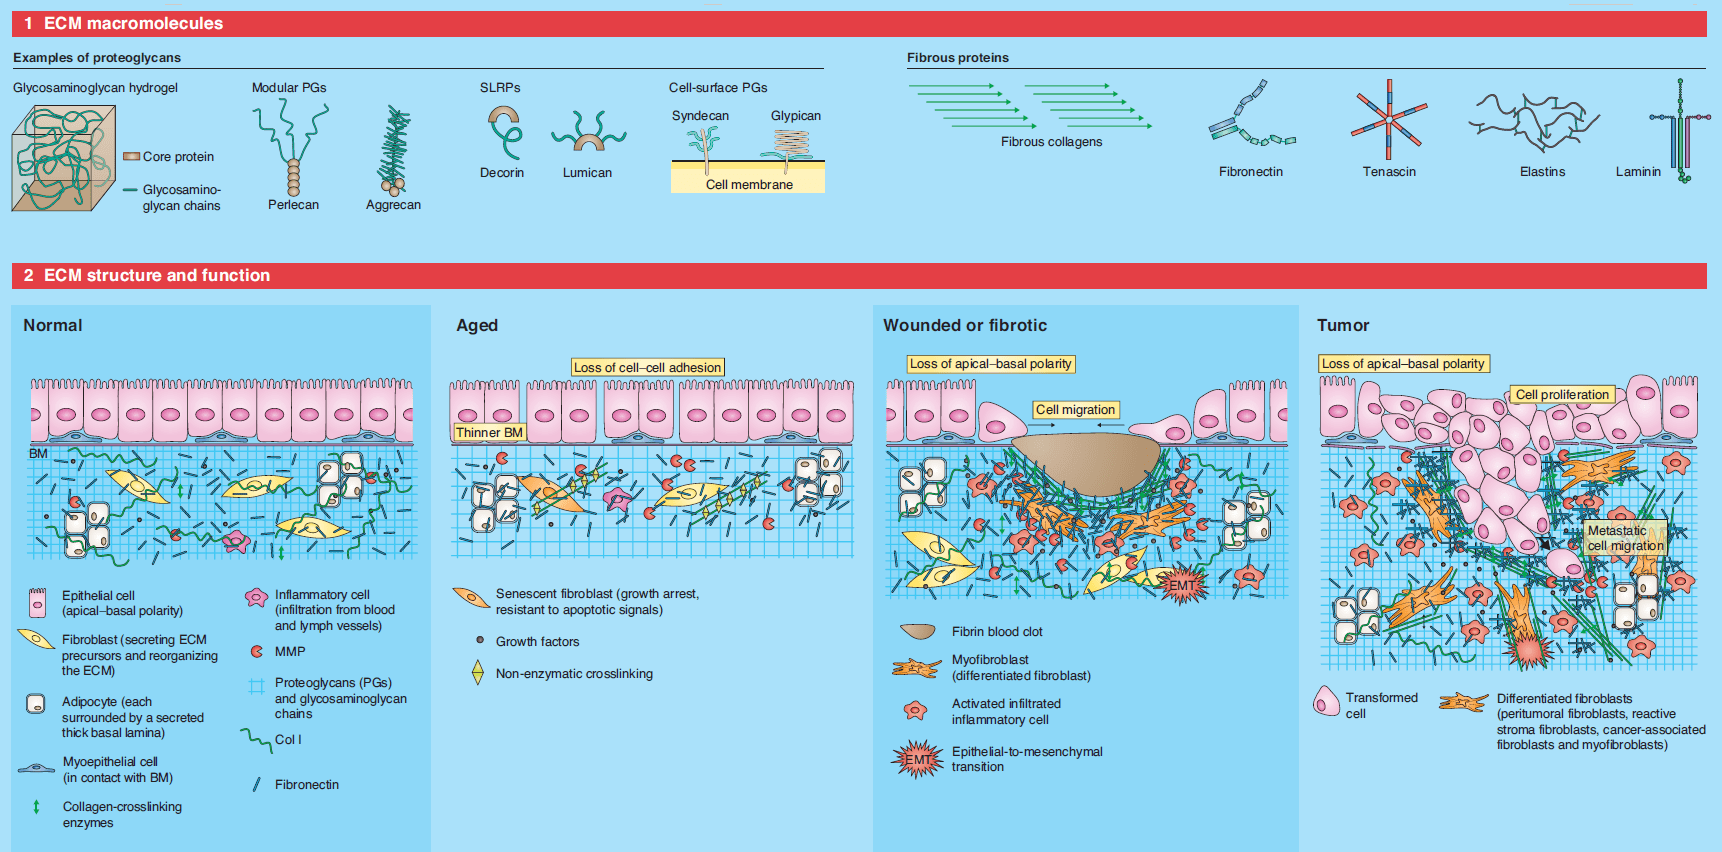
\includegraphics[width=1\textwidth]{ECMfunction.png}
		\caption{\label{fig:ECM} ECM functionalization}
		\end{figure}
		\noindent
		Figure \ref{fig:ECM}:the first example is a normal situation, good substrate. In an aged person we have a loss of elasticity. In the case of a wound, we observe a coagulation cascade and scar tissue formation - which is characterized by a compact tissue. The temporary material (crust) is used as scaffold. We can have healing by repair or regeneration. There is a higher rigidity in the case of temporary material. In the case of a tumour, we have an abnormal growth and migration inside - which they should not be present. The migration is caused by fibers not organising to close the hole.

	\subsection{Surface chemistry: biorecognition in the ECM}
	Cell biology is governed by a complex series of interactions with the ECM.
	It is not enough to promote proliferation, the adhesion involving integrins should also be controlled.
	A pool of molecules is needed, since biological functions are orchestrated by a symphony of signals.
	Communication between cells and the cellular matrix is relevant in the regeneration process.

	\subsection{Biomaterials}
	A biomaterial is a substance that has been engineered to take a form which, alone or as a part of a complex system, is used to direct, by control of interactions with components of living systems, the course of any therapeutic or diagnostic procedure in human or veterinary medicine.
	The aim is to recreate a basic environment before inducing regeneration.
	Proliferation must be upregulated at the beginning to create a population.
	Once the right quantity of cells are in place proliferation needs to be stopped to produce a functional ECM and achieving a therapeutic impact.

	\subsection{Cell - molecules interactions}
	Cells can interact with moving molecules through the gap junctions or through integrins.
	These are sufficient to create communication between neighbouring cells, while travelling molecule are needed for communication between cells far from each other.
	The ECM should not allow for the degradation of these signalling molecules before they reach their target.

		\subsubsection{Maintaining the nutritional status}
		Nutritional status is the bottle neck of tissue engineering, because in big wounds it is difficult to provide nutrition.
		This is due to the fact that blood capillaries are missing from the injured site.
		Because of this, angiogenesis must be promoted early in regeneration.
		Hydrogels are an ideal material for promoting angiogenesis because they provide a favourable environment for angiogenesis while providing mechanical support.

		\subsubsection{Cell language}
		The cell language is based on a mapping between micro and nano pattern of the biopolymers that constitute the dynamic nature of the ECM and the receptors on cells that are their complementary binding.
		During cell activity the chemical processes are:

		\begin{multicols}{2}
			\begin{itemize}
				\item Irreversible chemical reactions that provide free energy (ATP $\rightarrow$ ADP) to the cells.
				\item Reversible shape changes in the ECM's biopolymers that provide control over the chemical reactions.
			\end{itemize}
		\end{multicols}

	\subsection{Biocompatible materials: foundation ideas}
	In order to design suitable materials, the biological pathways that lead to normal healing and reconstruction should be known.
	Secondly, it is required to develop bio recognition surfaces that turn these pathways on and off.
	To do so, it is necessary to know specific affinities for the key molecules found in healing wounds that are associated with vascularised healing and regeneration triggering unnatural local healing.
	If biomolecules are immobilised at the surface, they must be in the correct orientation and conformation.
	Porosity should be engineered to induce vascularisation and decrease the production of fibrotic tissue.
	Furthermore, the modulus matching of scaffold-biomaterial should match with their intended use: modulus mismatch should exacerbate the FBRx.
	Lastly, the engineered scaffold should be able to degrade into non-reactive substances at predetermined degradation rates to serve as a temporary guide for healing.

\section{Cell interactions}
Cells interact with the environment thanks to soluble factors, the extracellular matrix and receptors.
Signals come from the ECM and from neighbouring cells:

\begin{multicols}{2}
	\begin{itemize}
		\item Gene expression regulation leads to adult stem cell differentiation into the lineage of interest.
		\item Tissue specific differentiation.
		\item Survival of primary cells.
		\item interaction with apoptosis: under external stimuli the cells may go to apoptosis.
			This may be useful in case of chemotherapy.
	\end{itemize}
\end{multicols}

	\subsection{Cell adhesion}

		\subsubsection{Molecular mechanism}
		The orientation of ligands is critical for cell adhesion and biological function.
		The RGD sequence promotes cell adhesion and it is usually included in a long peptide so to avoid cell-cell adhesion.
		Depending on the protocol parameters, a nice or absent adhesion can be obtained changing adhesion proteins' orientation.
		This is due to a different density of signal, leading to a different outcome in adhesion.
		When designing a scaffold, the aim is to reach an adhesion equilibrium.
		Decreasing the signal density could allow cell movement, promoting migration into the scafffold.
		A stronger signal could promote a fast formation of a cell layer.
		No protein absorption into the scaffold means that there will be no adhesion.
		This can be useful in some cases, for example to avoid thrombus formation in blood vessels or to release cancer treatments from nanoparticles.
		It is clear how cell adhesion depends on the scaffold's surface, the conformation and orientation of which can be controlled through cell sensors or screening.

		\begin{figure}[h]
		\centering
		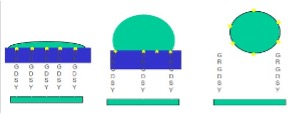
\includegraphics[width=0.5\textwidth]{adhesion}
		\caption{\label{fig:adhesion}}
		\end{figure}

		\subsubsection{Biological process}
		Cell adhesion is a tightly regulated and dynamic biological process.
		It is central to physiological and pathological processes and critical to biomedical and biotechnological applications.
		Adhesive interactions involve:

		\begin{multicols}{2}
			\begin{itemize}
				\item Anchorage that promotes migration and tissue organisation.
				\item Signalling that promotes activation, survival, proliferation and differentiation.
			\end{itemize}
		\end{multicols}

		\subsubsection{Some example of functional tissue assembling}

		\begin{figure}[h]
		\centering
		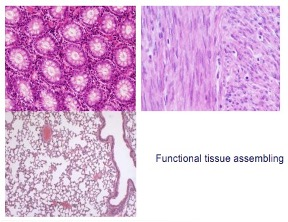
\includegraphics[width=0.5\textwidth]{functionaltissue}
		\caption{\label{fig:funtis}}
		\end{figure}

		In figure \ref{fig:funtis} starting from top left the functional tissue assembling of the radial section of glands , muscles, and lung/alveolar tissue can be seen.
		In the case of muscles, functional tissue should support mechanical stress.
		In glands cells are forming very well polarized capillary tubes for transport.
		For lung tissue blood vessels are present, a small surface and permeability for gas exchange are necessary.
		The air should move into the bloodstream, so the tissue should be very thin and adherent to the vessels.
		There is a low amount of ECM, with the mechanical support is provided by cells themselves.
		It is clear from these examples how the structure is function-dependent.
		Assembly is driven by ECM and adhesion patterning.
		The morphology should depend on the function: for example the thin layer of ECM in the basal lamina formed of collagen fibrils not organized in the classical bundles provides elasticity.

		\subsubsection{Difference between 2D and 3D adhesion}
		Adhesion is completely different in 2D and 3D.
		Cell adhesion is characterized by three stages:

		\begin{multicols}{2}
			\begin{itemize}
				\item Attachment of the cell body.
				\item Flattening and spreading.
				\item Organization of the actin skeleton with the formation of focal adhesion between cell and its substrate.
			\end{itemize}
		\end{multicols}

		The strength of adhesion becomes stronger with the time a cell is allowed to adhere.

	\subsection{Cell - ECM interaction}
	The interaction between cells and matrix can be compared to a chemical reaction where reagents can give rise to a reaction in a specific condition.
	The reactants are the cell and the matrix.
	The reaction takes place only if there is biorecognition: the interaction between cells and the ECM, often mediated by integrins.
	In order to achieve regeneration a number of functionalities must be activated at precise moments.
	The scaffold is a reactant and it is added in the reaction like mechanical stresses.
	The control system should not be downregulated: once the tissue has been regenerated the process must stop.

	\begin{figure}[h]
	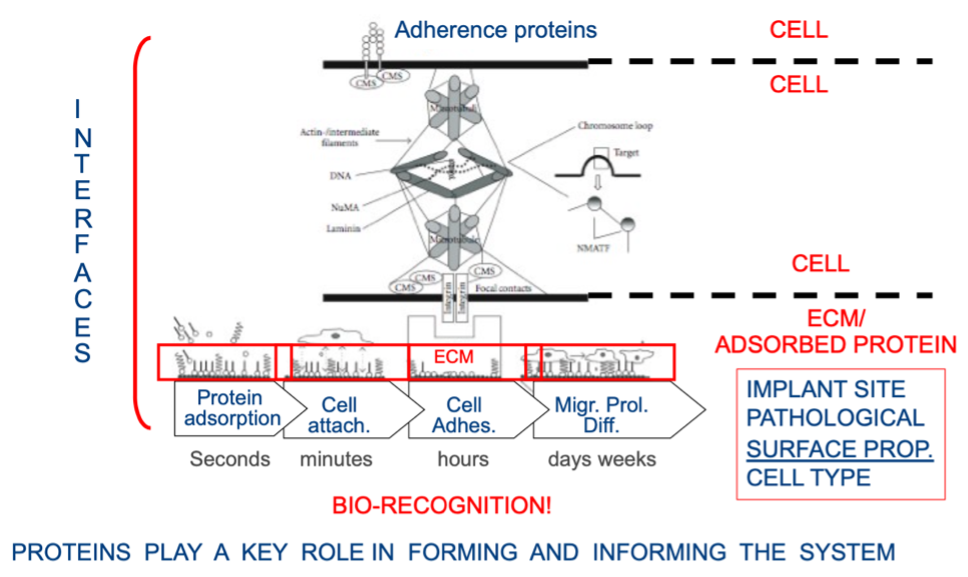
\includegraphics[width=1\textwidth]{interfaces}
	\caption{\label{fig:interfaces}}
	\end{figure}

	\subsection{Cell - scaffold interaction}
	Cells are in suspension in a culture with proteins.
	When the scaffold is inserted in the culture it absorbs a coating of ions, proteins and lipids, which are recognized and bound by cells.
	Which proteins will be absorbed depends on the chemical and mechanical properties of the scaffold and the context of implantation.
	The first absorbed proteins will be taken by plasma when bleeding occurs.
	The cells will adhere through integrins if they find ligands in the absorbed proteins.
	Cell adhesion happens only when biorecognition of the scaffold occurs.

		\subsubsection{Scaffold surface}
		Surfaces must be designed in order to control protein absorption.
		Depending on the phenotype of the adherent cells, different integrins will be needed.
		The aim when designing a scaffold is to promote cell adhesion through specific integrins so to achieve regeneration.
		Scaffolds and cells are not isolated: the empty spaces between them will be filled by the ECM which will provide proteins and water.
		This adhesion step will determine the failure or the success of the scaffold, making its surface really relevant for its function.
		To achieve the correct surface the scaffold can be functionalized through new chemical groups and its morphology can be changed to drive the interaction between scaffold and cells.

		\subsubsection{Protein absorption}
		The interaction between the implant and biological systems is a dynamic process.
		The biomaterial is characterized by specific properties.
		If the material is incubated in a single protein solution, where the protein is in active conformation, depending on the surface properties, the biomaterial will absorb the proteins, which will remain active, or we will witness deactivation, degradation or modification.

		\begin{multicols}{2}
			\begin{itemize}
				\item Absorption with original conformation: active protein.
				\item Denaturation during absorption: deactivation of the protein.
				\item Absorption with different conformation: different activity, which could lead to unexpected situations.
				\item Degradation: no specific activity, negative response and inflammation, causing the release of small pro-inflammatory peptides are released into the environment.
			\end{itemize}
		\end{multicols}

		The state of the protein is dependent on the scaffold aim.
		This absorption process is dynamic and protein can be released after they are absorbed.

		\subsubsection{Protein substrate}
		The protein substrate is important for the scaffold's functionality.
		By changing the material different interactions with proteins can be observed.
		Biocompatibility is a two-way process, the host affects the implant and vice versa.
		Differential adhesion distribution could be observed between domains.

		\subsubsection{Some example of scaffold - cell interaction}

			\paragraph{Polyurethane - an example}

			\begin{figure}[h]
				\centering
				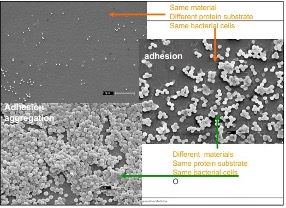
\includegraphics[width=0.5\textwidth]{polyu}
				\caption{\label{fig:polyu}}
			\end{figure}

			In the experiment depicted in figure \ref{fig:polyu} the aim was to produce a surface avoiding bacterial infection.
			The polymer used is polyurethane, used for catheter production where antibacterial properties are really required.
			The surface in contact with different protein substrates leads to different adhesion levels.
			When instead the protein substrate is equal with different materials, adhesion or adhesion aggregation can be seen.

			\paragraph{Vascular graft}

			\begin{figure}[h]
				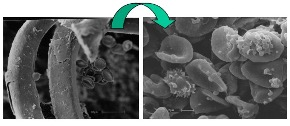
\includegraphics[width=0.5\textwidth]{vascular}
				\centering
				\caption{\label{fig:vascular}}
			\end{figure}

			Figure \ref{fig:vascular} depicts a vascular graft that failed after 6 years of implantation.
			The implant failed because the surface was completely destroyed.
			Bacterial cells  adhered to the implant and activated an inflammatory response.
			Inflammatory cells digested the implant, made of polyester.
			In addition, the implant started to detach in the circulation system  and bacteria were able to attach to red blood cells.
			This is one of the few cases in which we do not want cell adhesion.

		\subsubsection{Cell adherence on the scaffold}
		Cells cannot adhere to synthetic surfaces, as there is no biorecognition and the competition of the ECM is to strong.
		Cell adhesion to synthetic and bio surfaces occurs through a specific receptor interaction with adhesion protein/motifs:

		\begin{multicols}{2}
			\begin{itemize}
				\item Proteins adsorbed from physiological fluids like fibronectin, vitronectin or fibrogen.
				\item ECM components present or deposited by cells like fibronectin, collagen or laminin.
				\item Biospecific sequences engineered on surfaces like RGC or YIGSR for biorecognition.
			\end{itemize}
		\end{multicols}

		Adhesion receptor families are cadherins, selecting, HSPG, integrins and the Ig superfamily.
		Specific integrins act on specific receptors, so there is a need for precision.
		For instance, $\alpha 5\beta 3$ can recognize the ligands into fibronectin, while collagen is recognized by $\alpha 2 \beta 1$.

			\paragraph{Quantifying the adhesion strength}
			To measure adhesion strength, centrifugation of a sample is performed and the cells that remain attached to the scaffold are counted.

			\paragraph{Cell adhesion rate}
			Depending on the surface chemistry, there will be different cell adhesion rate.
			According to the protein coating, different biological performances will be visible.
			A number of evaluation methods can give us an idea of the adherence strength.

			\paragraph{Scaffold for neuron regeneration - an example}
			Figure \ref{fig:fibrin} depicts a designed scaffold for neuron regeneration.
			Adhesion is necessary, but neurons also need to form connections with other neurons.
			The RGD goal is neurite outgrowth, obtained through RGD functionalization.
			The material was provided with fibrin with different level of RGD, the classical adhesion peptide.

			\begin{figure}[h]
				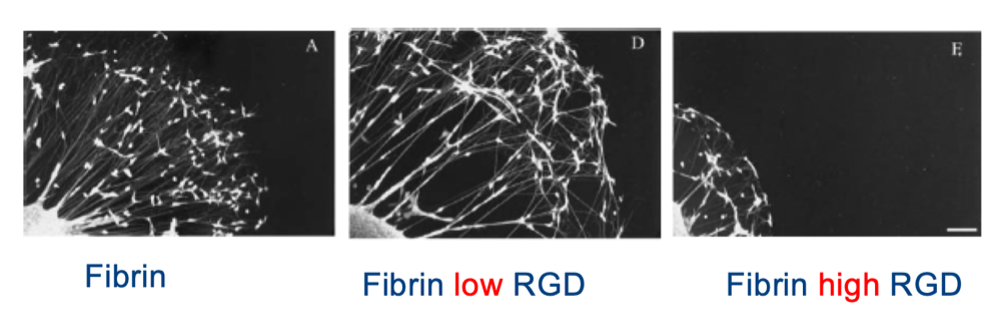
\includegraphics[width=1\textwidth]{fibrin}
				\caption{\label{fig:fibrin}}
			\end{figure}

			A different response is observed: a good outcome is obtained with a low amount of RGD with a huge number of connections.
			Increasing RGD causes the surface to become more adhesive making the cells to sticky.
			The amount of RGD should resemble the natural one.
			In fibronectin, the RGD content is 1 per chain.
			It is clear here how signal is the combination of the specific ligand and its density.


	\subsection{Cell organization}
	Cells' adhesive interactions with the surrounding ECM defined by the number of adhesive motifs, their distribution and their density and neighbouring cells define cell shape and organisation, controlling functionality.
	This environment regulates the cell survival, differentiation, proliferation and migration.

		\subsubsection{Some examples}

			\paragraph{Chondrocytes}
			Chondrocytes are exposed to compressive forces with an interstitial fluid flow and adhesive cues given by cytokines for cartilage maintenance.
			Chondrocytes are found in a lacuna, where they should behave like pillars and maintain their shape.

			\paragraph{Blood vessel wall}
			Soluble and matrix-bound GFs and flow induced mechanical forces on blood vessel wall, cause cell-cell contacts, and degrade the surrounding basement membrane and stromal ECM in order to migrate and form tubular sprouts.
			Adhesive and mechanical cues drive cell organization.

			\paragraph{Epithelial cells}
			Misregulation of the mechanism induces mechanical and structural changes in the ECM, and transformed epithelial cells migrate towards vasculature and eventually metastasize.

		\subsubsection{ECM controls adhesion and migration}
		ECM-dependent regulators can be associated with 2D, 1D and 3D migration, that in turns influences intracellular pathways that govern the migratory phenotype.
		3D migration is defined by pore size and interconnection, the cross linking degree.
		Aligned fibers are randomly distributed with low density in the scaffold.
		Adhesion and migration are controlled by the ECM composition, stiffness of the material and ligand density.
		An aligned topography of fibres allow to obtain different architectures.
		In the case of a mixed fibrous scaffold, aligned and random, fibres are present with an elastic behaviour, exacerbated by cross linking.
		Sending seed cells on the different structure, diverse behaviour for orientation, migration, proliferation, growth and differentiation will be obtained.
		Architecture can play a huge role in scaffold functionality.

			\paragraph{Contractility}
			The substrate contractility regulates 3D migration, regardless of pore size.
			When a cell lands on a stiff fiber it can adhere, but it becomes very stable and not able to modify its shape or migrate.
			Instead, cells on soft fibers are able to move and form protrusions.
			Since cells in nature are connected to ECM fibers, when they move the ECM will also follow the contraction of the cell body.
			If the cell adheres to soft fibers, the same natural movement can occur.
			When the substrate is too rigid contraction cannot occur and healing will be different.
			The scaffold should be soft enough to follow the reorganization needed by the cells.

			\paragraph{Mineralization}

			\begin{figure}[h]
				\centering
				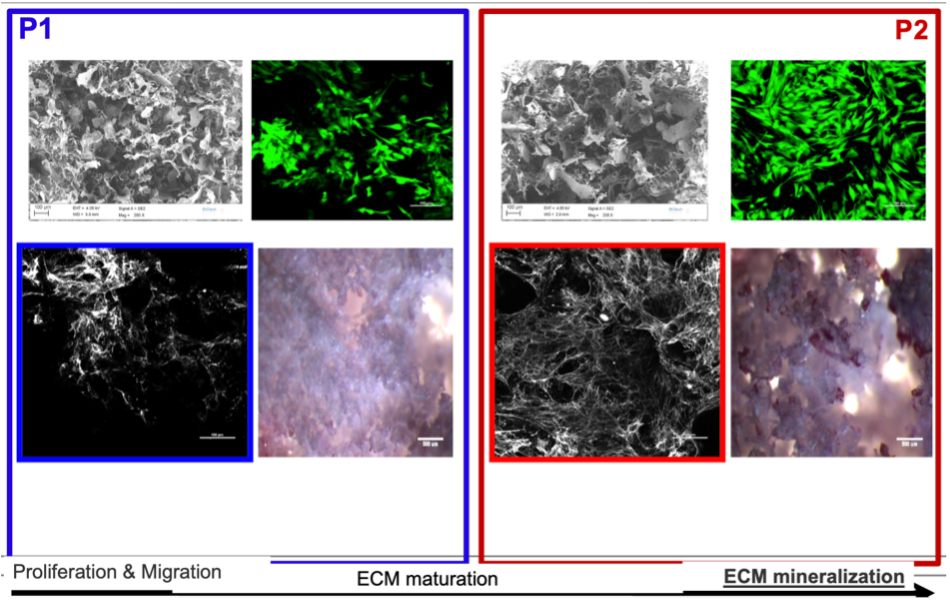
\includegraphics[width=0.7\textwidth]{mineralization}
				\caption{\label{fig:min}}
			\end{figure}

			Figure \ref{fig:min} depicts two scaffolds prepared with the same polymer but different for pore size and distribution.
			The scaffolds are built for bone regeneration: the presence of collagen fiber in a continuous network should be considered.
			Osteoblasts should infiltrate the scaffold for building the network and the porosity should allow this.
			Once the network is formed, hydroxy apatite is deposited on top of the collagen fibers.
			While in P2 the cell distribution is uniform, in P1 it is clustered because interconnection is not complete.
			These clusters don't allow a continuous network to be built due to tight collagen and the lack of mineralization.
			In fact when cells are not able to migrate, mineralization cannot occur.

			\paragraph{Capillary formation}
			A continuous network is required for capillary formation.
			The parameters can be fully controlled with scaffold design.
			In order to improve the performance of the P2 scaffold we could functionalize it with collagen or drug release systems.

		\subsubsection{Reproducing in vitro a working environment}
		The scaffold surface interacts with the cell through the ECM during biorecognition.
		The aim is to reproduce in vitro a working environment, working for the cell and solving a specific task.
		Depending on the context, the bioreaction can happen: the cell recognizes the surface of the scaffold if it is functionalized or for protein absorption.
		Cell population, and integrins, are context specific.

	\subsection{Methods for modulating receptor-ligand interactions}
	To modulate receptor-ligand interactions, one could control:

	\begin{multicols}{2}
		\begin{itemize}
			\item Natural ECM biomaterials: biologically relevant environment, but poor mechanical properties and inconsistent reproducibility.
			\item Whole ECM adsorption.
			\item Synthetic linear binding motif: surface functionalization.
				There is a need to define the density of the signal, the protein of interest, the stability (quantify the time for which the signal should remain), orientation, homogeneous or pattern distribution.
			\item Spatially oriented binding motif.
			\item Nanopatterning with nanolithography: mix different molecules and patterns, as well as technologies.
			\item ECM-like biomaterials.
		\end{itemize}
	\end{multicols}

\section{Biorecognition requirements}
The biorecognition process will have a good outcome only if the absorbed proteins are the right ones according to the following parameters:

	\subsection{Absorbed protein recognition}
	The absorbed proteins must contain sequences (ligands) recognizable by dedicated cellular receptors: among the first we remember RGD, YIGSR, IKVAV and RETTAWA, among the second we cite integrins.
	Integrins are heteromeric transmembrane receptors that mediate cell - ECM interaction with different glycoproteins among whom fibronectin and vitronectin and collagen fibers.

	\subsection{Ligand orientation}
	The ligands mentioned above must be oriented outward, they must not be hidden or used by the scaffold to link with the proteins.
	If this happens, the sequences won’t be able to be recognized by the cellular receptors.

	\subsection{Stability}
	The absorbed proteins must have a stable structure: they must not denature, take on conformations with unexpected functions like prions or hold native functions that could hinder the regenerative process like trigger clotting formation or release peptides that could be pro-inflammatory, leading to chronic inflammation.

	\subsection{Concentration}
	The array of absorbed protein must expose the right number of ligands, with the right density.
	In particular for the regenerative aim, the ligands need to be in the right number and density to allow for macrophage adhesion while still allowing them to move.
	They need also to stretch across the binding sites, since this stretching has been correlated with the polarization towards the M2 phenotype for macrophages.
